\chapter{OBJECT RECONSTRUCTION AND SAMPLE SELECTION}
\label{sec:EventReconstruction}

\section{Overview of the CMS reconstruction process}
\label{sec:recoOverview}

For each event that passes the trigger, the output from all of the sub-detectors described in Chapter~\ref{chap:Detector} is saved by the data acquisition system (DAQ) and eventually recorded to disk and tape. The data format at this stage is referred to as ``RAW" data. It includes information about the response of each detector, but the data are still unprocessed, aside from the minimal processing done to determine whether the event passed the trigger. ``Reconstruction" is the general term for algorithms that convert the detector response data into lists of object candidates---muons, photons, electrons, jets, etc.---and event quantities such as missing transverse momentum \ptmiss. 

Figure~\ref{fig:cmsSlice} shows how each type of particle interacts with the different layers of the CMS detector. Photons, being neutral, do not interact with the tracker, and deposit their energy in the ECAL. Electrons have a very similar response in the ECAL, but unlike photons, they also leave hits in the tracker. Hadrons deposit their energy in the HCAL, and charged hadrons have an associated track in the tracker. Finally, muons interact with the tracker and the muon system. 

 \begin{figure*}[h!]
	\centering
	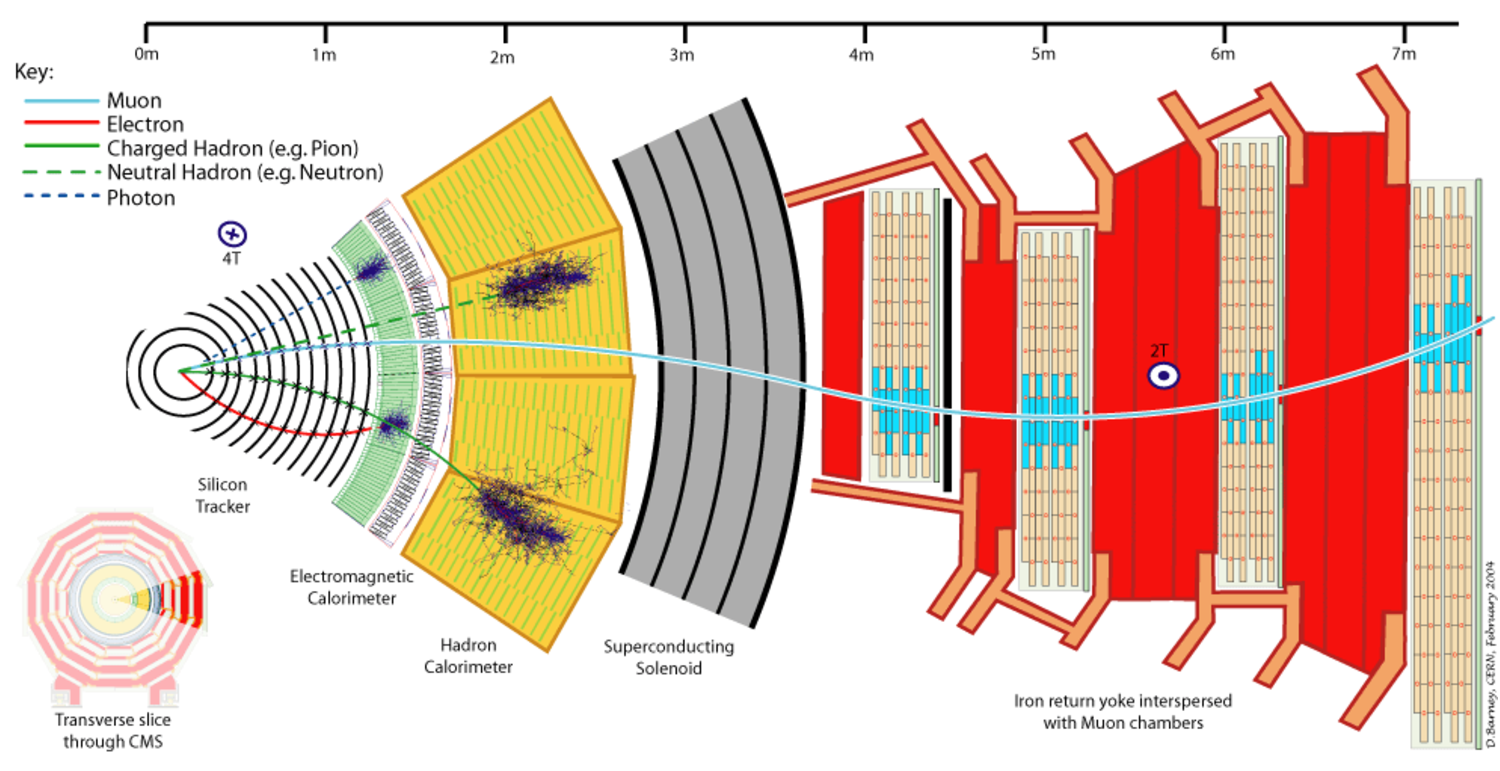
\includegraphics[width=\linewidth]{Figures/EventReconstruction/cms_slice.pdf}
       \caption{Slice of the transverse plane of the CMS detector showing how different particles interact with the detector subsystems. The most important particle for this analysis is the photon (blue dotted line), which interacts only with the ECAL (shown in green).
       Reprinted from Reference~\cite{CDS}.}
       \label{fig:cmsSlice}
\end{figure*}

Of course, the simplified picture in Figure~\ref{fig:cmsSlice} does not cover the full complexity of how particles can interact with the detector. Photons can ``convert" and produce an electron-positron pair. Hadrons can interact with the material of the tracker or ECAL, and begin to shower before reaching the HCAL. The following sections will describe in more detail how physics objects are reconstructed. 

%%%%%%%%%%%%%%%%%%%%%%%%%%%%%%%%%%%%%%%%%

\section{Particle flow algorithm}
\label{sec:ParticleFlow}
CMS uses a ``particle-flow" (PF) reconstruction algorithm \cite{ParticleFlow}. The PF approach seeks to assign each hit in the tracker and each calorimeter energy deposit (known as a cluster) to a final-state particle. This holistic view maximizes our ability to identify particles by using the full set of information provided by the detector. CMS is the first hadron accelerator experiment to use PF for reconstruction. It is made possible through the excellent spatial resolution of the tracker and calorimeters and the large bending power of the magnet. Both of these features are necessary so that signals from nearby particles do not overlap. For example, the ECAL cluster from a charged particle with $\pT =$ 20 GeV will be deviated by 5 cm from the ECAL cluster of a neutral particle emitted in the same direction, allowing the two particles to be reconstructed independently \cite{ParticleFlow}.

The ingredients to the PF algorithm are reconstructed tracks and calorimeter clusters. The relevant algorithms and methods for each of these elements will be discussed first, before describing how they are assembled to form the final lists of candidate photons, electrons, muons, and jets. 

\subsection{Track reconstruction}
\label{sec:trackReco}
Tracking in CMS takes place with a combinatorial track finder that is applied in ten iterations. The iterations use successively more complex algorithms with looser requirements on the track properties. Each iteration includes three basic steps:
\begin{itemize}
\item Seed generation: The first step is to find a track seed consisting of two or three hits compatible with a charge-particle track.
\item Track finding: Pattern recognition is used to identify hits in all layers of the tracker that are compatible with the trajectory implied by the track seed. 
\item Track fitting: A global $\chi_2$ fit is performed to determine the final properties of the track, including origin, direction, and transverse momentum. 
\end{itemize}

Because the charged particles can change direction suddenly through interactions with the tracker material, the track finder uses a Kalman filter method~\cite{Kalman}. The goal of each iteration is to find tracks with as high of a purity as possible, at the cost of moderate efficiency. The high purity is accomplished through quality cuts on the seeds and the $\chi_2$ of the track fit. Any hits that are associated with a track are masked for the subsequent iterations. This reduces the combinatorial possibilities, which in turn reduces the likelihood of random hits being built up into a fake tracks. 

In addition to particle identification and determination of transverse momentum, tracks are also used to reconstruct vertices in the event. 
The vertex with the largest value of $\Sigma\pT^2$ is identified as the primary vertex, associated with the hard-scatter interaction. The other vertices arise from soft-scatter pileup interactions. Thus, the number of reconstructed vertices in an event can be used to approximate the number of pileup interactions. Two of the later iterations of the track finder are applied with reduced constraints on the origin vertex, in order to reconstruct displaced secondary vertices from the decays of long-lived particles. 

Specialized algorithms are used to reconstruct tracks for electrons and muons. Those are described in detail next.

\subsection{Electron track reconstruction}
\label{sec:eleTrackReco}

Electrons have a higher probability of scattering in the tracker than other charged particles, and so electrons are reconstructed using a separate tracking algorithm that is optimized for multiple scatters. In particular, a Gaussian-sum filter (GSF) is used rather than a Kalman filter because it adapts better in the case of sudden and substantial momentum changes. Two approaches are used: an ECAL-driven approach and a tracker-driven approach. In the ECAL-driven method, ECAL clusters are used to infer the hit locations assuming that the cluster came from either a positron or an electron. 

The tracker-driven method is better for electrons in jets and for low-\pt electrons, when the ECAL clusters are overlapping with deposits from other particles or are too spread out to reconstruct fully. In this approach, all tracks with \pt greater than 2 GeV are used as seeds for an electron. Each track is propagated to the surface of the ECAL and checked to see if it is consistent with the position of an ECAL cluster. The final step of the algorithm uses a boosted decision tree (BDT) to quantify the goodness of fit. This last step serves to reduce the misidentification rate, which is especially important in the context of the PF algorithm to avoid double counting energy.

\subsection{Muon track reconstruction}
\label{sec:muonTrackReco}
PF muons are classified into three categories:
\begin{itemize}
\item All reconstructed tracks with $\pt > 0.5$ GeV and $|\vec{p}| > 2.5$ GeV in the inner tracker are propagated to the muon system, and classified as \textbf{tracker muons} if they match at least one hit in the muon section. 
\item \textbf{Standalone muons} are reconstructed using the muon system only. The process starts with seed tracks in the DT or CSC detectors, and a pattern recognition algorithm identifies DT, CSC, and RPC hits corresponding to the muon trajectory.
\item \textbf{Global muons} are standalone muons that are consistent with a track in the inner tracker. 
\end{itemize}

Because of the extensive amount of material that muons must traverse before reaching the muon system, the inner tracker gives the best energy resolution for muons up to 200 GeV \cite{ParticleFlow}.

\subsection{Reconstruction of calorimeter clusters}
\label{sec:clusterReco}
Calorimeter clusters are an important input for the PF algorithm. They are the sole means of detection for photons and neutral hadrons, and they are essential for improving the energy resolution of electrons and high-\pt jets. The reconstruction of a cluster begins with a ``seed" cell (ECAL crystal or HCAL scintillating tile) that corresponds to a local energy maxima above a given threshold. Starting from the seed cell, topological clusters are formed by adding cells that share a side or corner with the cluster and have an energy that is at least twice the noise threshold. For the EB, the seed energy must be greater than 230 MeV, and subsequent crystals must have an energy of at least 80 MeV in order to be added to the topological cluster. Finally, a fit is performed to determine what fraction of the energy in the cell is associated with each PF cluster, where the number of PF clusters is equal to the number of seeds incorporated into the topological cluster.

The ECAL clusters are calibrated for photons and electrons using test beam data and radioactive sources, and residual corrections are derived using single photon MC samples. For hadrons, however, the ECAL must be re-calibrated, since the response of the ECAL to hadrons is significantly different than its response to electrons. A large simulated sample of neutral hadrons is used to derive a simultaneous calibration for the portions of the hadronic shower's energy deposited in the ECAL and HCAL. 

One complication in the reconstruction of ECAL clusters is the presence of signals known as spikes. These occur when a particle directly ionizes an ECAL APD. The result is a signal whose amplitude is $10^5$ times higher than the signal from the scintillation light alone. Because these spikes appear in only one or two crystals, they are rejected by considering the ratio of energy deposited in the central crystal to that deposited in the neighboring 4 crystals. In the case where the spike affects two adjacent crystals, the energy deposited in the two crystals is compared to that of their six neighbors. These ratios are referred to as $E_4/E_1$ and $E_6/E_2$, and are required to be less than 5\% and 10\%, respectively. 

\subsection{Particle identification}
\label{sec:partID}
A ``link" algorithm is used to connect tracks and calorimeter clusters and quantify the likelihood that two elements arose from the same particle. A dedicated procedure is used to link tracks with any ECAL clusters that are consistent with photons from electron bremsstrahlung  and to link two tracks compatible with a photon conversion. A group of linked elements is referred to as a PF block. 

Particle flow is an iterative procedure. As object candidates are identified within a PF block, their corresponding tracks and clusters are removed from further consideration. This makes PF different from more traditional reconstruction algorithms where clusters or hits could be attributed to more than one particle. The object-identification process is repeated until all tracks and clusters have been assigned to a single PF candidate. 

First, muon candidates are identified with two sets of identification criteria: one for isolated muons and one for muons inside or near jets. Next, electron candidates and photon candidates are reconstructed. Finally, any remaining tracks or calorimeter clusters in the PF block are assigned to a neutral hadron, charged hadron, or photon candidates.

Because photons are the primary object of interest in this analysis, their reconstruction is described in more detail below. 

\section{Photon identification}
\label{sec:phoReco}




%https://www3.nd.edu/~cjessop/talks/JessopCMS101.pdf
The reconstruction of photon clusters with a seed as defined in Section~\ref{sec:clusterReco}. The ratio of the energy in a 3 $\times$ 3 array of crystals to that in a $5 \times 5$ region is referred to R9. If R9 is greater than 0.93, than the photon is classified as unconverted, and the energy of the 5 $\times 5$ region is assigned as the photon super-cluster energy. If the photon has converted (ie, R9 $< 0.93$), then the super-cluster is built starting with the seed crystal and moving outward.




%%%%%%%%%%%%%%%%%%%%%%%%%%%%%%%%%%%%%%%%%

\section{Jet reconstruction}
\label{sec:Jet}
Jets are reconstructed from PF candidates using the \antikt algorithm with a distance parameter $R =$ 0.4~\cite{antikt}.  The \antikt algorithm is a sequential clustering algorithm where the distance $d_{ij}$ between two particles $i$ and $j$ and the distance $d_{iB}$ between particle $i$ and the beam $B$ are given by the following: 
\begin{equation}
\begin{aligned}
d_{ij} &= \mathrm{min}(k_{ti}^{2p},k_{ti}^{2p})\frac{\Delta^2_{ij}}{R^2} \\
d_{iB} &= k_{ti}^{2p}
\end{aligned}
\end{equation}

The value $\Delta^2_{ij}$ is equal to $(\eta_i - \eta_j)^2 + (\phi_i - \phi_j)^2$, $k_t$ is the transverse momentum of the particle, and $R$ is a distance parameter that determines the final radius of the jet.

The clustering algorithm first finds the smallest value of $d_{ij}$ and $d_{iB}$ for all particles in the event. If the minimum distance is $d_{ij}$, then particles $i$ and $j$ are combined into a single entity. If the minimum distance is $d_{iB}$, then particle $i$ is labeled a jet and removed from the list. For the \antikt algorithm, the parameter $p = -1$. Setting $p=0$ corresponds to the inclusive Cambridge/Aachen algorithm, and $p=1$ is the inclusive $k_t$ algorithm. The result of various jet-clustering algorithms is shown in Figure~\ref{fig:jetAlgorithms}. One obvious feature of the \antikt algorithm is the production of very circular jets compared to jets identified using other clustering algorithms.
 
 \begin{figure*}[h!]
	\centering
	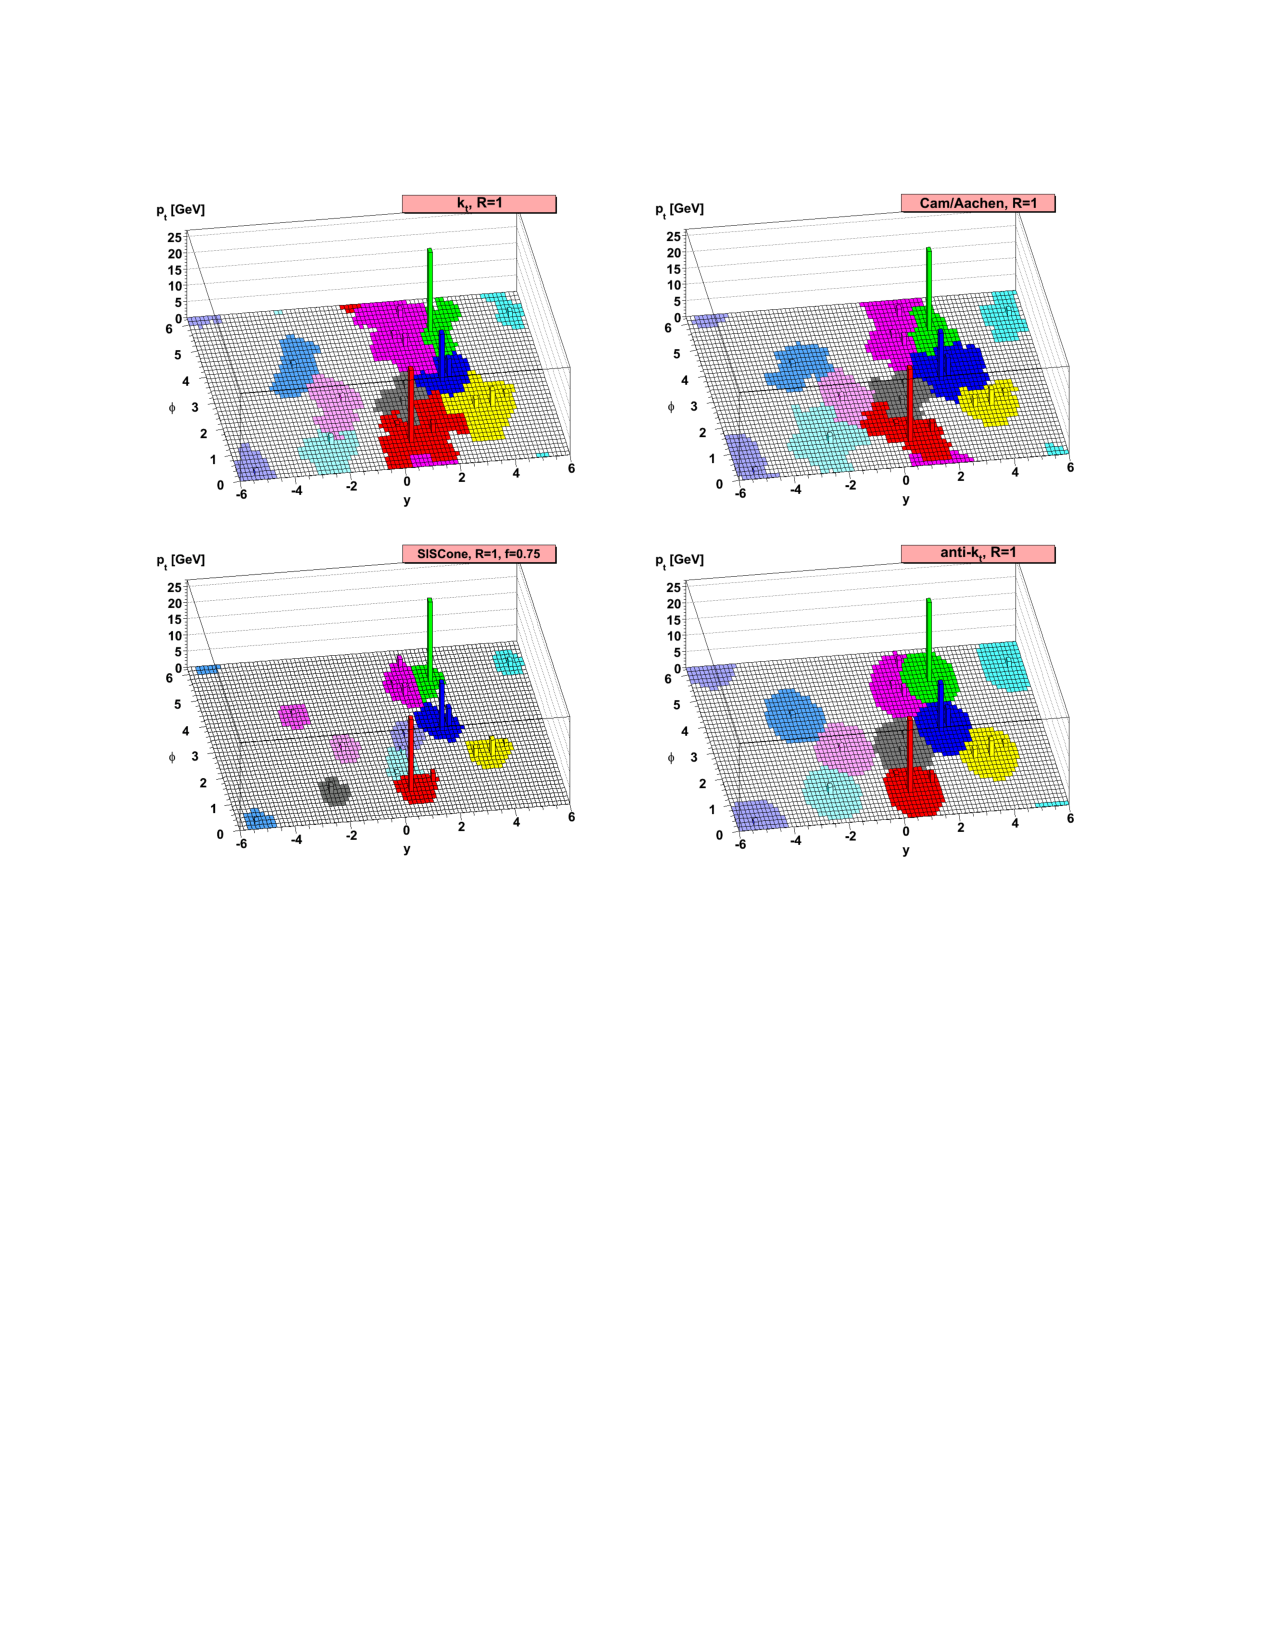
\includegraphics[width=\linewidth]{Figures/EventReconstruction/jetAlgorithms.pdf}
       \caption{Behavior of several jet-clustering algorithms illustrated with a sample parton-level event. 
       CMS uses the \antikt algorithm (bottom right) with a distance parameter $R = 0.4$.
       Reprinted from Reference~\cite{antikt}.}
       \label{fig:jetAlgorithms}
\end{figure*}
 
One benefit of the \antikt algorithm is that it is infrared and collinear (IRC) safe. Infrared safe means that \antikt jets are insensitive to nearby soft particles. In the \antikt algorithm, soft particles (those with $k_t \rightarrow 0$) have a large $d_{ij}$ and are therefore clustered last. This leaves hard jets unaffected. Soft particles could possibly by clustered into many soft jets, but those are simple to remove during the analysis. Being infrared safe is particularly important for the high luminosity environment of the LHC, so that the clustering of the hard jets from the primary interaction is not changed by the many soft particles from pileup interactions.

Collinear safe means that very energetic initial quarks will still get reconstructed as a single jet. In the \antikt algorithm, collinear particles will have a small value of $\Delta^2_{ij}$ and will be clustered together first. Using an IRC safe algorithm is important for comparing theory and experiment, because if jets are not IRC safe, then their cross sections cannot be calculated using perturbation theory.

\subsection{Jet energy corrections}
\label{sec:JEC}

A series of jet energy corrections (JEC) are applied to the jets after clustering to improve the calibration and energy resolution \cite{JEC}. The $L1$ correction is a flat correction designed to remove contributions to the jet energy from pileup (see Section~\ref{sec:pileup} for a more thorough description of pileup mitigation techniques). The $L2$ corrections are $eta$-dependent and the $L3$ corrections are \pt-dependent. These are calculated in simulation using generator truth information. In data, the correction factors are derived using dijet events and events where a jet is emitted back-to-back with an photon. In the latter case, the superior energy resolution of the ECAL is exploited to provide a handle on the jet energy. The effects of JEC on jet response in QCD MC is shown in Figure~\ref{fig:JEC}.

 \begin{figure*}[h!]
	\centering
	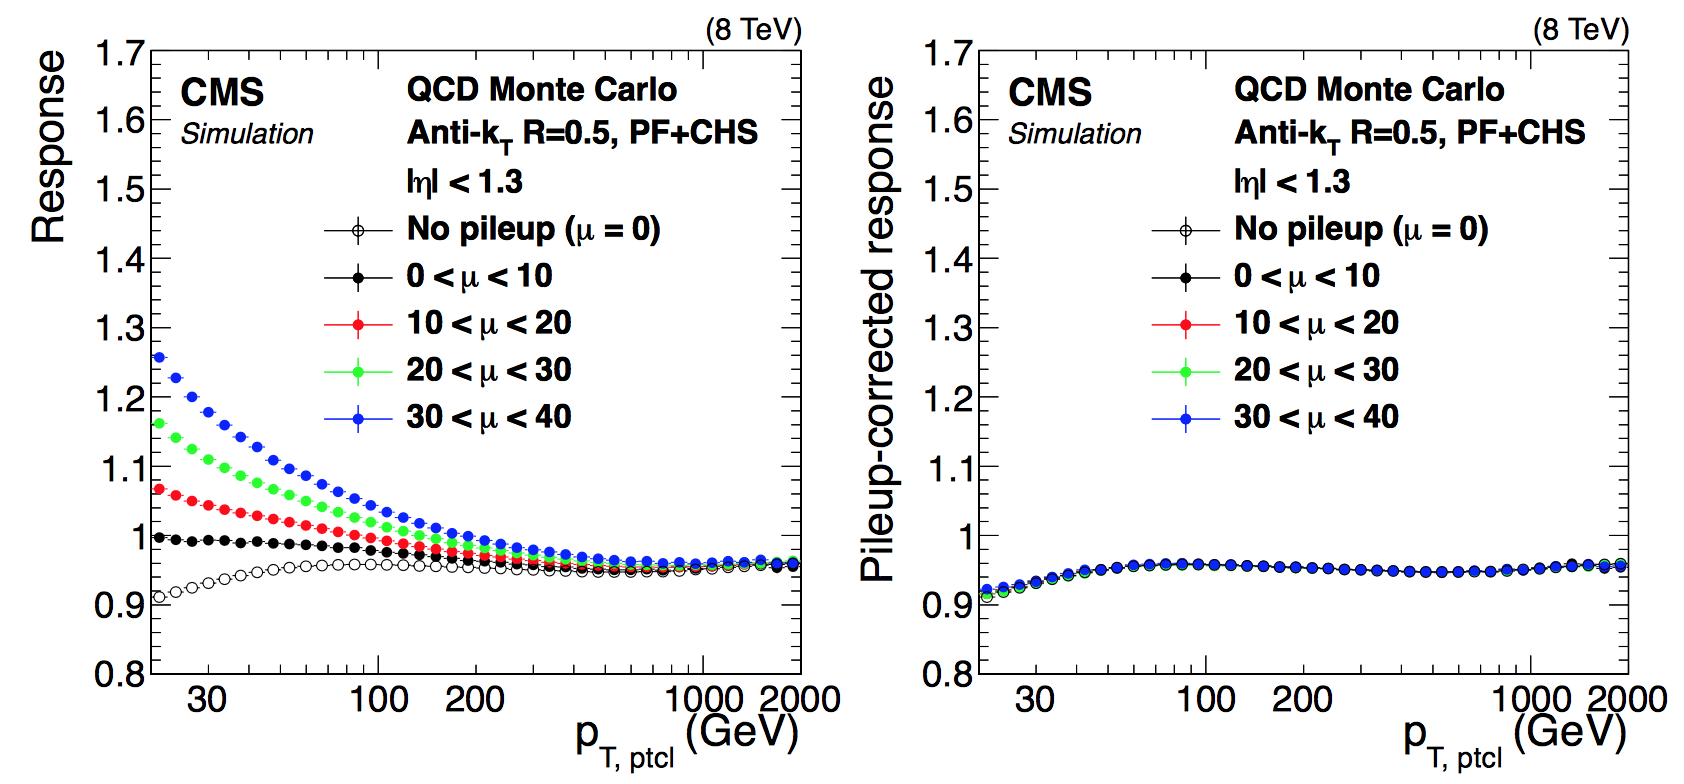
\includegraphics[width=1.0\linewidth]{Figures/EventReconstruction/JEC1.png}
	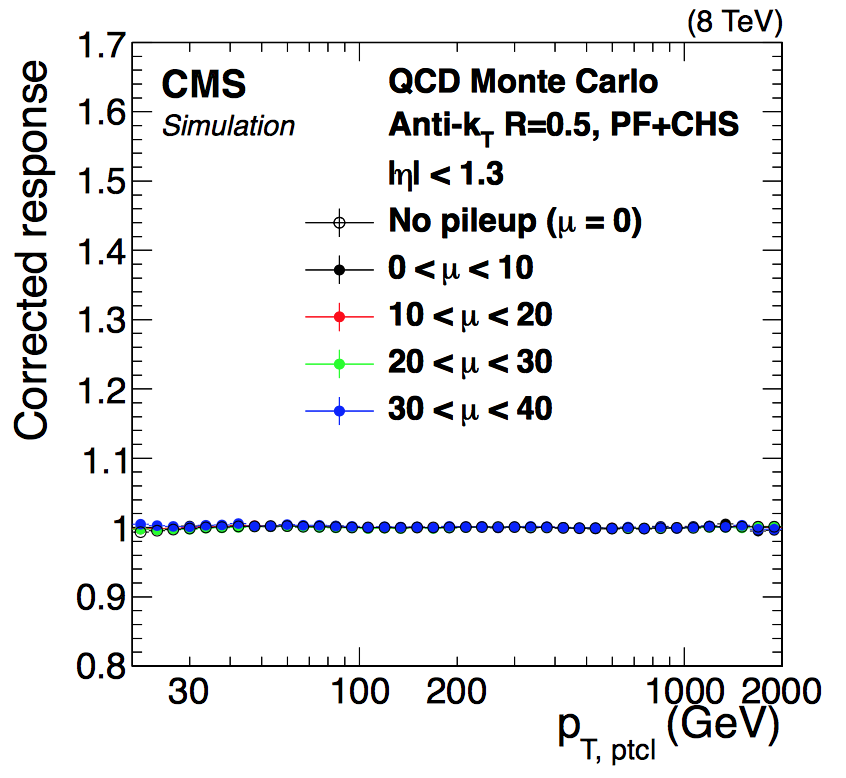
\includegraphics[width=0.5\linewidth]{Figures/EventReconstruction/JEC2.png}
       \caption{Ratio of the average reconstructed jet \pt to the particle-level jet \pt ($p_{\mathrm{T,ptcl}}$) in QCD MC simulation.
       The ratio is calculated in bins of $p_{\mathrm{T,ptcl}}$ before applying any JEC (top left), after applying the $L1$ pileup corrections
       (top right), and after all JEC (bottom). The different curves correspond to different numbers of pileup interactions $\mu$.
       Reprinted from Reference~\cite{JEC}.}
       \label{fig:JEC}
\end{figure*}

\subsection{Jet energy resolution}
\label{sec:JER}

After the JEC are applied, resolutions of 10\% and 5\% are achieved for 100 GeV and 1 TeV jets in the barrel, respectively. Figure~\ref{fig:JER} shows the jet energy resolution as a function of jet \pt in 8 TeV simulation. 

 \begin{figure*}[h!]
	\centering
	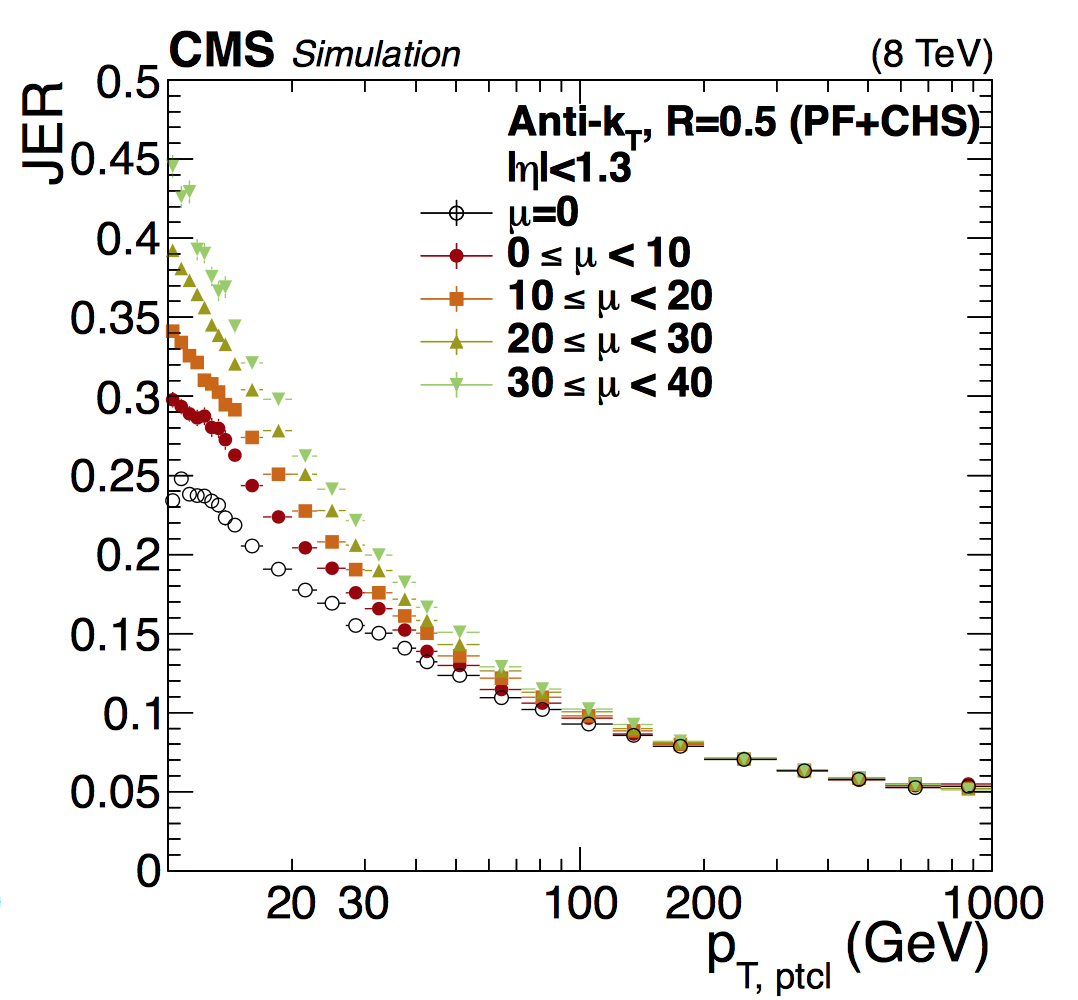
\includegraphics[width=0.65\linewidth]{Figures/EventReconstruction/JER.png}
       \caption{Jet energy resolution (JER) in 8 TeV simulation as a function of particle-level jet \pt ($p_{\mathrm{T,ptcl}}$). PF+CHS refers to particle-flow
       jets with charged hadron subtraction (see Section~\ref{sec:pileup}). Results are shown for various levels of pileup $\mu$. 
       Reprinted from Reference~\cite{JEC}.}
       \label{fig:JER}
\end{figure*}

%%%%%%%%%%%%%%%%%%%%%%%%%%%%%%%%%%%%%%%%%

\section{Missing transverse momentum}
\label{sec:MET_Reco}
After the full set of PF objects have been identified and reconstructed, the missing transverse momentum $\vec{\pt}^{\mathrm{miss}}$ is given by the following, where the sum is over all Particle Flow objects:
\begin{equation}
\vec{\pt}^{\mathrm{miss}} = \Sigma \ptvec
\end{equation}
The magnitude of this quantity is referred to as the missing transverse energy \ETmiss. For the calculation of \ETmiss in this analysis, Type-I corrections are applied, which correspond to propagating the JEC described above to the \ETmiss. 

There are several situations that can arise where particle misidentification or poor reconstruction leads to an artificially large value of \ETmiss. These are dealt with in post-processing by substituting the reconstructed particles with alternative hypotheses and checking how the \ETmiss changes. For example, very energetic charged hadrons can occasionally punch through the HCAL and leave tracks in the muon system. In this case, PF will reconstruct a neutral hadron and a muon, leading to a large value of $\vec{\pt}^{\mathrm{miss}}$ pointing in the opposite direction. If replacing the neutral hadron and muon with a charged hadron reduces the \ETmiss by 50\% or more, then that alternative reconstruction is used instead.

In addition to the post-processing corrections just described, a series of \ETmiss filters are applied. The filters are designed to tag events where the \ETmiss is poorly reconstructed. At the analysis stage, if an event fails any of the \ETmiss filters it is removed from consideration. The following \ETmiss filters applied in this analysis:
\begin{itemize}
\item Primary vertex filter
\item CSC beam halo filter
\item HBHE noise filter
\item HBHEiso noise filter
\item ECAL trigger primitive filter
\item ee badSC noise filter
\item Bad PF muon filter
\item Bad charged hadron filter
\item Duplicate muons filter
\end{itemize}

%%%%%%%%%%%%%%%%%%%%%%%%%%%%%%%%%%%%%%%%%

\section{Pileup subtraction}
\label{sec:pileup}

The presence of pileup interactions affects many aspects of the reconstruction process, in particular the jet energy resolution, lepton isolation values, and \ETmiss. Fortunately, there are several ways in which the PF algorithm can be used to mitigate the effects from pileup. Charged-hadron subtraction (CHS), for example, is the procedure of removing charged hadrons from consideration if they are associated with a pileup vertex rather than the hard-scatter vertex. Figure~\ref{fig:jetComp} shows the composition of jets in data and simulation as a function of the number of pileup interactions $\mu$. For an event with $\mu = 30$, 10\% of the uncorrected jet energy is due to charged hadrons from pileup interactions. 

 \begin{figure*}[h!]
	\centering
	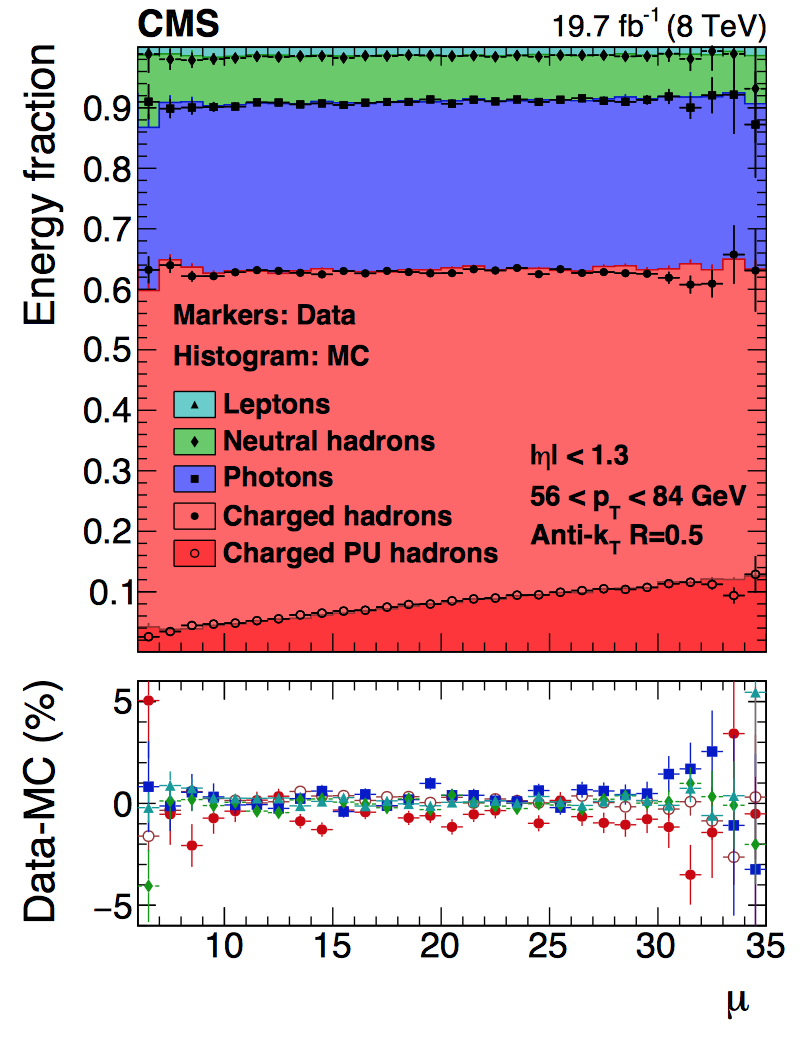
\includegraphics[width=0.65\linewidth]{Figures/EventReconstruction/jetComp.png}
       \caption{Energy composition as a function of the number of pileup (PU) interactions $\mu$ for jets in 
       data (markers) and simulation (histogram). The data distributions correspond to 19.7\fbinv collected at 
       $\sqrt{s} = 8$ TeV with the CMS detector in 2012.
       The contribution from charged hadrons from pileup is shown in dark red.
       The bottom pane shows the agreement between data and MC for each category.
       Reprinted from Reference~\cite{ParticleFlow}.}
       \label{fig:jetComp}
\end{figure*}

The pileup contributions from photons and neutral hadrons, however, cannot be subtracted on an object-by-object basis, since there is no good way to identify whether these neutral particles were produced in the primary interaction or in a pileup interaction. These effects can only be subtracted from the event on average. For lepton and photon isolation, this is done by calculating $\rho$, the \pt density due to pileup interactions \cite{XX}. The average contribution to the isolation sum from pileup is then given by $\rho$ times the effective area of the object under consideration. The calculation of the effective areas for photons and electrons is described in Reference~\cite{XX}.


